\documentclass{llncs}

\usepackage{fuzz}
\usepackage{courier}
\usepackage[usenames,dvipsnames]{xcolor}
\usepackage{tikz}
\usepackage{eufrak}
\usepackage{imakeidx}
\newcommand{\dindex}[1]{\index{#1|textbf}}
\newcommand{\theme}[1]{\emph{#1}\dindex{#1}}  
\usepackage{hyperref}
\hypersetup{
    colorlinks,
    citecolor=green,
    filecolor=green,
    linkcolor=blue,
    urlcolor=green
}
\usepackage{wrapfig}

\usetikzlibrary{arrows,automata,snakes,arrows,shapes,calc,positioning}
\tikzstyle{accept}=[fill=gray]
\tikzstyle{skip}=[rectangle,draw=black]
\tikzstyle{next}=[circle,draw=black,minimum size=5mm]
\tikzstyle{quant}=[rectangle,dashed,draw=black,minimum size=5mm]
\tikzset{initial text={}}


\usepackage{amsmath,amssymb}

\usepackage{graphicx}
\usepackage{pgfplots}
\usepackage{graphics}
\usepackage{placeins}
\usepackage{subfigure}
%\usepackage{kpfonts}

\usepackage{color}
\definecolor{light-gray}{gray}{0.95}

\newcommand{\name}[1]{\texttt{#1}}

\newcommand{\ignore}[1]{}

\newcommand{\GR}[1]{\notethis{ForestGreen}{Giles}{#1}}
\newcommand{\GRinline}[1]{{\color{ForestGreen}{#1}}}
\newcommand{\KH}[1]{\notethis{blue}{Klaus}{#1}}
\newcommand{\KHinline}[1]{{\color{blue}{#1}}}

\newcommand{\notethis}[3]{
  \color{#1}
  \vspace{0.3cm}
  \noindent\makebox[\linewidth]{\rule{\paperwidth}{0.4pt}}\\
  {\sc #2 - } #3\\
  \noindent\makebox[\linewidth]{\rule{\paperwidth}{0.4pt}}\\
  \vspace{0.3cm}
  \color{black}
}
\newcommand{\todo}[1]{{\color{red}{#1}}}

\newcommand{\red}[1]{{\color{red} #1}}
\newcommand{\green}[1]{{\color{green} #1}}
\newcommand{\blue}[1]{{\color{blue} #1}}
\newcommand{\orange}[1]{{\color{orange} #1}}

\usepackage{listings}

\lstdefinelanguage{scala}{
  morekeywords=
    {package,import,class,object,trait,extends,with,match,
     new,if,else,while,for,yield,def,val,var,this,case,
     type,implicit,private,protected,abstract,final}, 
  literate=
      {=>}{{$\Rightarrow$ }}2
      {\#\#}{{$\oplus\;$}}2
      {|->}{{$\longmapsto\;$}}2
      {-->}{{$\Longrightarrow\;$}}2
      {->}{{$\rightarrow\;$}}2
      {>>}{{$\gg$}}2
      {++}{{$++$}}2
      {|==}{{$\models$}}2
  ,
  sensitive=true, 
  morecomment=[l]{//}, 
  morecomment=[s]{/*}{*/},
  escapeinside={(*}{*)},
  stringstyle=\ttfamily,
  %aboveskip=1mm,
  %belowskip=1mm,
  showstringspaces=false,
  columns=flexible,
  morestring=[b]",
  %basicstyle={\scriptsize},
  %numbers=left,
  numberstyle=\scriptsize,
  %moredelim=[is][\bf\em]{|}{|},
  %moredelim=[is][\bf\em]{+}{+},
  moredelim=[is][\em]{@}{@}
} 

\lstdefinelanguage{oclinecore}{  
morekeywords={class,invariant,self,attribute,property,derived,derivation,operation,body,select,forAll}, 
  literate=
      {->}{{$\rightarrow\;$}}2
      {<=}{{$\le$}}2
  ,
  sensitive=true, 
  morecomment=[l]{//}, 
  morecomment=[s]{/*}{*/},
  escapeinside={(*}{*)},
  stringstyle=\ttfamily,
  %aboveskip=1mm,
  %belowskip=1mm,
  showstringspaces=false,
  columns=flexible,
  morestring=[b]",
  %basicstyle={\scriptsize},
  %numbers=left,
  numberstyle=\scriptsize,
  %moredelim=[is][\bf\em]{|}{|},
  %moredelim=[is][\bf\em]{+}{+},
  moredelim=[is][\em]{@}{@}
} 

\lstdefinelanguage{zlang}{
  morekeywords=
    {}, 
  literate=
      {->}{{$\rightarrow\;$}}2
      {<=}{{$\le$}}2
      {Int}{{$\mathbb{Z}$}}2
      {String}{{$\mathbb{C}^*$}}2
  ,
  sensitive=true, 
  morecomment=[l]{//}, 
  morecomment=[s]{/*}{*/},
  escapeinside={(*}{*)},
  stringstyle=\ttfamily,
  %aboveskip=1mm,
  %belowskip=1mm,
  showstringspaces=false,
  columns=flexible,
  morestring=[b]",
  %basicstyle={\scriptsize},
  %numbers=left,
  numberstyle=\scriptsize,
  %moredelim=[is][\bf\em]{|}{|},
  %moredelim=[is][\bf\em]{+}{+},
  moredelim=[is][\em]{@}{@}
} 

\lstdefinelanguage{klang}{
  morekeywords=
    {class, req}, 
  literate=
      {->}{{$\rightarrow\;$}}2
      {<=}{{$\le$}}2
  ,
  sensitive=true, 
  morecomment=[l]{//}, 
  morecomment=[s]{/*}{*/},
  escapeinside={(*}{*)},
  stringstyle=\ttfamily,
  %aboveskip=1mm,
  %belowskip=1mm,
  showstringspaces=false,
  columns=flexible,
  morestring=[b]",
  %basicstyle={\scriptsize},
  %numbers=left,
  numberstyle=\scriptsize,
  %moredelim=[is][\bf\em]{|}{|},
  %moredelim=[is][\bf\em]{+}{+},
  moredelim=[is][\em]{@}{@}
} 

\lstdefinelanguage{vdm}{
  morekeywords=
    {class,end,instance,variables,functions,types,operations,inv,
    public,
    token,set,of,map,to,nat,
    forall,exists,in,dom,and,let,be,st,return,card,
    pre,post}, 
  literate=
      {->}{{$\rightarrow\;$}}2
      {==>}{{$\Rightarrow$}}2
  ,
  sensitive=true, 
  morecomment=[l]{//}, 
  morecomment=[s]{/*}{*/},
  escapeinside={(*}{*)},
  stringstyle=\ttfamily,
  %aboveskip=1mm,
  %belowskip=1mm,
  showstringspaces=false,
  columns=flexible,
  morestring=[b]",
  %basicstyle={\scriptsize},
  %numbers=left,
  numberstyle=\scriptsize,
  %moredelim=[is][\bf\em]{|}{|},
  %moredelim=[is][\bf\em]{+}{+},
  moredelim=[is][\em]{@}{@}
}

\newcommand{\scala}{\lstset{language=scala,backgroundcolor=\color{white}, frame=none,basicstyle={\small}}}
\newcommand{\iscala}{\scala\lstinline} % inline scala

\newcommand{\scalaimpl}{\lstset{language=scala,backgroundcolor=\color{white}, frame=none,basicstyle={\small}}}

\newcommand{\oclinecore}{\lstset{language=oclinecore,backgroundcolor=\color{white}, frame=none,basicstyle={\small}}}
\newcommand{\iocl}{\oclinecore\lstinline} % inline ocl

\newcommand{\zlang}{\lstset{language=zlang,backgroundcolor=\color{white}, frame=none,basicstyle={\small}}}

\newcommand{\klang}{\lstset{language=klang,backgroundcolor=\color{white}, frame=none,basicstyle={\small}}}

% -------
% Themes:
% -------

\newcommand{\oldtheme}[1]{\emph{#1}}

\newcommand{\THsafetyliveness}{\theme{Safety versu Liveness}}
\newcommand{\THnames}{\theme{Statemachines}}
\newcommand{\THreachability}{\theme{Reachability}}
\newcommand{\THnonregularity}{\theme{Non-regularity}}
\newcommand{\THsequences}{\theme{Sequences}}
\newcommand{\THtemporallogic}{\theme{Temporal Logic}}
\newcommand{\THconvenient}{\theme{Convenient operators}}
\newcommand{\THquantification}{\theme{Quantification}}
\newcommand{\THtiming}{\theme{Time}}
\newcommand{\THcoding}{\theme{Coding}}
\newcommand{\THmatching}{\theme{Matching}}
\newcommand{\THembedding}{\theme{Embedding}}
\newcommand{\THscope}{\theme{Scope}}
\newcommand{\THalphabet}{\theme{Alphabet}}
\newcommand{\THmodularity}{\theme{Modularity}}

\newcommand{\THdomains}{\oldtheme{Domains}}
\newcommand{\THlocalglobalstate}{\oldtheme{Local vs. Global State}}
\newcommand{\THpolarity}{\oldtheme{Polarity}}
\newcommand{\THsuffix}{\oldtheme{Prefix or Suffix}}
\newcommand{\THmixinglogics}{\oldtheme{Mixing Logics}}
\newcommand{\THparameters}{\oldtheme{Parameters}}
\newcommand{\THexistential}{\oldtheme{Existential Quantification}}
\newcommand{\THspecialCase}{\oldtheme{Special Case}}
\newcommand{\THskipnext}{\oldtheme{Skip or Next Semantics}}
\newcommand{\THpast}{\oldtheme{Past time logic}}
\newcommand{\THtimelines}{\oldtheme{Timelines}}
\newcommand{\THlanguagespecific}{\oldtheme{Language Specific}}

%Splitting aggregates
\newcommand{\THcounting}{\theme{Aggregates (counting)}}
\newcommand{\THsum}{\theme{Aggregates (sum)}}
\newcommand{\THaverage}{\theme{Aggregates (average)}}


\newcommand{\logfire}{{\sc LogFire}}
\newcommand{\qea}{{\sc qea}}
\newcommand{\marq}{{\sc MarQ}}
\newcommand{\larva}{{\sc Larva}}
\newcommand{\scala}{{\sc Scala}}
\newcommand{\rete}{{\sc Rete}}
\newcommand{\ruler}{{\sc Ruler}}
\newcommand{\drools}{{\sc Drools}}
\newcommand{\clips}{{\sc Clips}}
\newcommand{\jess}{{\sc Jess}}
\newcommand{\hammurabi}{{\sc Hammurabi}}
\newcommand{\rooscaloo}{{\sc Rooscaloo}}
\newcommand{\tracecontract}{{\sc TraceContract}}
\newcommand{\daut}{{\sc Daut}}
\newcommand{\java}{{\sc Java}}
\newcommand{\mop}{{\sc Mop}}
\newcommand{\mac}{{\sc Mac}}
\newcommand{\salt}{{\sc Salt}}
\newcommand{\timeedit}{{\sc TimeEdit}}
\newcommand{\psl}{{\sc Psl}}
\newcommand{\eagle}{{\sc Eagle}}
\newcommand{\hawk}{{\sc Hawk}}
\newcommand{\jlo}{{\sc Jlo}}
\newcommand{\tracematches}{{\sc TraceMatches}}
\newcommand{\metatem}{{\sc MetateM}}
\newcommand{\logscope}{{\sc LogScope}}
\newcommand{\haskell}{{\sc Haskell}}
\newcommand{\mopbox}{{\sc MopBox}}
\newcommand{\orchids}{{\sc Orchids}}
\newcommand{\ltlfoplus}{{\sc LTL-FO}$^+$}
\newcommand{\xml}{{\sc Xml}}
\newcommand{\mfotl}{{\sc MFOTL}}
\newcommand{\ltlfo}{{\sc LTL}$^{\rm FO}$}
\newcommand{\prolog}{{\sc Prolog}}
\newcommand{\jpax}{{\sc Jpax}}
\newcommand{\python}{{\sc Python}}
\newcommand{\rmor}{{\sc Rmor}}
\newcommand{\scalatest}{{\sc ScalaTest}}
\newcommand{\ltl}{{\sc Ltl}}
\newcommand{\temporalrover}{{\sc TemporalRover}}
\newcommand{\staterover}{{\sc StateRover}}
\newcommand{\aspectj}{{\sc AspectJ}}
\newcommand{\vdmpp}{VDM$^{++}$}



\title{Towards a Unified View of\\ Modeling and Programming }

\author{
Manfred Broy\inst{1}
\and
Klaus Havelund\inst{2}\thanks{The research performed by this author was carried out at Jet Propulsion Laboratory, California Institute of Technology, under a contract with the National Aeronautics and Space Administration.}
\and 
Rahul Kumar\inst{3}
}
\institute{
Technische Universit{\"a}t M{\"u}nchen, Germany
\and
Jet Propulsion Laboratory, California Inst. of Technology, USA 
\and
Microsoft Research, USA
}
\makeindex[title=Themes]

\begin{document}
\maketitle

\begin{abstract}
In this paper we argue that there is a value in providing a 
unified view of modeling and programming. Models are meant to
describe a system at a high level of abstraction for the purpose of
human understanding and analysis. Programs, on the other hand, 
are meant for execution. However, programming languages are 
becoming increasingly higher-level, with convenient notation for 
concepts that in the past would only be reserved formal 
specification languages. This leads to the observation, that  
programming languages could be used for modeling, if only 
appropriate modifications were made to these languages.
At the same time, model-based engineering formalisms such as UML 
and SysML are highly popular in engineering communities due to 
their graphical nature. However, these communities are,
due to the complex nature of these formalisms, 
struggling to find grounds in textual formalisms with proper 
semantics. A unified view of modeling and programming may
provide a common ground. The paper illustrates these points 
with selected examples comparing models and programs.

\end{abstract}



\section{Introduction}
\label{sec:introduction}

Over the last several decades we have observed the development of a 
large collection of specification and modeling languages and 
associated methodologies, and tools. Their purpose is to 
support formulation of requirements and high-level designs before 
programming is initiated. Agile approaches advocate to avoid 
explicit modeling entirely and suggest to go directly to coding. 
Other approaches advocate avoiding manual coding in a 
programming 
language entirely and suggest instead the generation of code 
directly from the models. This way modeling languages replace 
programming languages.  We can divide modeling languages into 
formal specification languages (formal methods), usually focusing 
on textual languages based on mathematical logic and set theory, 
and associated proof tools (theorem provers, model checkers, etc.), 
and on the other hand model-based engineering languages (UML, 
SysML, Modelica, Mathematica, ...), focusing more on visual 
descriptions, code generation, and simulation. Many of these 
languages have similarities with programming languages.

In parallel, and frankly seemingly independent, we have seen the 
development of numerous new programming languages. Few languages 
have had the success of C, which still today is the main 
programming language for embedded systems. The success is so 
outstanding that nearly no progress wrt. praxis has been made in 
this domain (embedded programming) since the 1970ties, although 
some richer languages appeared soon after C in this domain, such as 
C++, Ada, and Eiffel. These later languages for example
all have module systems, which C does not. We have seen several high-level languages appear that target the softer side of software 
engineering (such as web-programming, user interfaces, scripting), 
including languages such as Java, JavaScript, Ruby, Python and 
Scala.  More academic languages include Haskell and the ML family, 
including OCaml.

There is seemingly a strict difference between a modeling
language and a programing language. For a
programming language we always assume a notion of {\em 
executability} and {\em computability}. Programming languages 
are restricted to concepts that can be
executed. Put differently, programming languages put emphasis on 
the {\em ``how''}, the algorithms for solving problems.
A specification and modeling language in principle should rather 
focus on the {\em ``what''}. A mathematical way of phrasing this is 
that specifications should ideally be {\em predicates} on solutions 
(executions for example). Intuitively, one may also argue that 
there are modeling tasks which do not directly aim at programing, 
for instance if we model a business process independent of the 
question which parts should be carried out by machines. This is 
modeling, which seems far away from programming. It might be 
interesting to bring it into a form which is closer to programming 
if we want to simulate or automatically analyze such models. But 
here there seems to be a boundary. Programming means computability. 
Modeling can be more general. Finally, at a more technical level, 
in programming, at least when we work in general purpose 
programming languages, we have to deal with non termination and the 
concept of undefined \cite{broy-chaos-2006}. 
In a number of modeling approaches such 
concepts like undefined are avoided. Here again 
there is an interesting challenge in a unifying
view of modeling and programming. We would have to manage to
introduce the concepts of undefined into modeling, representing
nonterminating expressions in programming.  Some attempts have been
made in	this direction though, for example 3-valued logic as 
found in VDM \cite{jones90}.

In spite of these perceived differences, the similarities between
modeling languages and programming languages are obvious, which
suggests a unifying view. For example, many logics support the 
notions of local variables with bounded scopes and syntactic 
expressions similar to programming languages. Many modeling 
languages even offer programming constructs, such as mutable 
variables, 
assignment statements, and looping (while) statements, and of course recursion. Furthermore, some of the modeling 
languages, such as UML, are deeply influenced by programming 
languages wrt. how models are structured. In particular, the idea 
of object-oriented modeling is taken from the concept of 
object-oriented programming. It is even considered one of the strong sides 
of object-orientation, that one can have a unified view of 
object-oriented specification, object-oriented design, and 
object-oriented programming. In summary, the concepts that 
are used in modeling and the concepts that are used in 
programming are so closely related that it is beneficial to attempt 
a unified view.

In this paper we attempt to argue for such a unified view 
of modeling and programming. This view can in the extreme be 
considered a call
for a single universal formalism for modeling and programming any
form of system. This is done by high-lighting some trends in 
modeling and programming, and by programming some example
models in the Scala programming language, a high-level formalism
suited for this purpose.
However, we fully understand that such a unification faces many
obstacles, some of which are non-technical. 
What we intend is to fuel an {\em effort} to at least consider
merging efforts to the extent feasible. We believe that the model-based
engineering community can learn from the formal methods and 
programming language communities, and vice versa. Note that even if a single
formalism would appear, there will always be alternatives, just like
there are multiple programming languages (evolution continues). 

The paper is organized as follows.
In Section \ref{sec:trends} we give a brief overview of some 
of the trends in modeling and programming, that we consider important. 
In Section \ref{sec:modeling-as-programming} we illustrate with examples how modeling can be perceived as programming. 
%In Section \ref{sec:concerns} we suggest discussion points to be reflected on
%when considering a unified approach.
Finally Section \ref{sec:conclusion} outlines
brief discussion points to be reflected on
when considering a unified approach, as well
as a conclusion.


\section{Trends in Modeling and Programming}
\label{sec:trends}

In this section we briefly survey some trends in the fields of
formal methods, model-based engineering, and programming, that we find worthwhile highlighting.


\subsection{Formal Methods}

Early work on formal methods include the work of John McCarthy 
({\em Recursive Functions of Symbolic Expressions and Their 
Computation by Machines} \cite{Mc60} and 
{\em Towards a Mathematical Science of Computation} \cite{Mc62a}), 
Robert Floyd ({\em Assigning Meanings to Programs} \cite{Flo67}), Edsger Dijkstra ({\em A Discipline of Programming} \cite{EWD1}), 
Tony Hoare ({\em An Axiomatic Basis for Computer Programming} \cite{Hoa69}), and Dana Scott and Christopher 
Strachey ({\em Towards a Mathematical Semantics for Computer 
Languages} \cite{Sco71}), to mention a few. These ideas were theoretic in nature and deeply influential. They brought us the ideas of  annotating programs with assertions, such as pre- and post-conditions, and invariants, correct by construction development (refinement), and giving semantics to programming languages. 

These ideas were subsequently the basis for several, what we could 
call, second generation formal specification languages such as 
VDM, Z, B, CIP, TLA, RAISE, and OBJ, to mention just a few. 
Each of these languages were full 
specification languages, most with rich type systems and detailed rules 
(grammars) for what constitutes a valid specification. These 
languages were ahead of their time wrt. language features in the 
sense that many of these features have found their 
way into modern programming languages of today. A particular
example of this is collections (sets, lists, and maps).

The VDM language for example is a wide-spectrum specification 
language offering a combination of high-level specification 
constructs and low level programming like constructs. The 
methodology 
consists in part, as in CIP, of refining a high-level specification 
into a low-level program like specification in a stepwise manner. 
The language offered concepts 
such as the combination of imperative (procedural and later 
object-oriented in \vdmpp) and functional programming; exceptions; 
algebraic data types and pattern matching; functions as values and 
lambda abstractions; built-in collection types such as sets, lists 
and maps, with mathematical notation for creating values of these 
types, such as for example set comprehension; design-by-contract 
through pre- and post conditions and invariants; predicate subtypes 
(so one for example can define natural numbers as a subset of the 
integers);  and predicate logic including universal and existential 
quantification over any type as Boolean expressions.  VDM and Z are 
so-called {\em model oriented} specification languages, 
meaning that a specification is an example model of the desired system. This means that such specifications are somewhat close to high-level programs. This is in contrast to so-called {\em property oriented} (algebraic) specification languages, such as OBJ, where a specification denotes a set of models\footnote{This characteristic of the difference is somewhat simplified since a VDM specification in fact also can denote more than one model.}.  

A different branch of formal methods includes theorem proving and 
model checking. In theorem proving we have seen specification 
languages, which resemble functional programming languages, 
including for example ACL, PVS and Coq. In model checking, early 
work focused on modeling notations somewhat removed from 
programming languages. However, recent research has focused on 
software model checking, where the target of model checking is 
code, as for example seen in the Java PathFinder model checker, 
JPF. JPF was created due to the observation that a powerful 
programming language might be a better modeling language than the 
traditional model checker input languages. Today’s 
efforts in model checking furthermore include numerous efforts in 
model checking of C programs.

As can be seen from the above discussion, formal specification 
languages have for a long time been flirting with programming 
language like notations, and vice versa. However, the two classes of languages have by tradition been considered as belonging to 
strictly separate categories. VDM for example was always, and still 
is, considered a specification language, albeit with code 
generation capabilities. It has never, in spite of the possibility, 
been named a programming language, which one may 
consider being as one of the reasons it is not more wide spread. 
Writing specifications in VDM and generating code in Java, for 
example, has not become popular. Programmers feel uncomfortable 
working with two languages (a specification language and  a 
programming language) when the two languages are too similar. This 
is an argument for merging the concepts into a  specification, 
design and implementation language.


\subsection{Model-based Engineering}

Model-based engineering includes modeling frameworks that are 
usually visual/graphical of nature. One of the main contributions 
in this field is UML for software development, and its derivatives, 
such as SysML for systems development. The graphical nature of the 
UML family of languages has caused it to become rather popular and 
wide-spread in engineering communities. Engineers are more willing 
to work with graphical notations, such as 
class diagrams and state machines, than they are working with sets, 
lists and maps and function definitions. It seems clearly more 
accepted than formal methods as described in the previous section. 
%At JPL for example, there are three people working with formal 
%methods and over hundred working with UML/SysML technology. 

One of the important notations in UML/SysML is class diagrams. 
Class diagrams are, just like E/R-diagrams, really a simple way 
of defining data, an alternative to working with sets, lists and 
maps as found in VDM and modern programming languages. For example, 
to state that a person can own zero or more cars one draws a box 
for Person, and a box for Car, and draws a line between them. It is 
an idea that quickly can be picked up by a systems engineer, 
quicker than learning to use programming language data structures. 
Another notation is that of state 
machines, a concept that interestingly enough has not found its way 
into programming languages, in spite of its usefulness in 
especially embedded programming. UML and SysML also support 
requirements (as special comments), a concept that usually is not embedded as a first citizen in programming. 
%It would be interesting to see requirements as part of programming.

The above observations are rather positive. However, UML and
SysML are very complex and weakly defined formalisms. 
For example, the combined syntax for all of UML corresponds 
to the sum of approximately 20 programming languages (approximately 
17,000 lines of abstract syntax, a programming language can 
normally be defined in between 500 and 2500 lines of grammar 
rules). The UML/SysML standards are long and complex documents. 
Furthermore, the connection between models and code is fragile, relying on the correctness of translators from for example UML state machines to code. Finally, a discussion about semantics
(what do two boxes with a line in between mean?) can turn 
a project meeting into chaos.


\subsection{Programming}

Several new programming languages have emerged over the last 
decades, which include abstraction mechanisms known from the formal 
specification languages mentioned above. Such languages include 
Eiffel, Java, Python, Scala, Julia, Fortress,  C\#, Spec\#, F\#,  Dafny, D, 
RUST, Swift, Go, Agda, and SPARK.  Some languages support 
design-by-contract with pre-post conditions, and in some cases with 
invariants. These languages  include for example Eiffel, Spec\#, 
Dafny, SPARK, and to some limited extent Scala. Java supports 
contracts through JML, which, however, is not integrated with Java, 
but an add-on comment language (JML specifications are comments in 
a Java program). Most of the languages above support abstract 
collections such as sets, lists and maps. It is interesting to 
observe that SUN’s Fortress language (which unfortunately was not 
finished due to lack of funding) supports a mathematical 
notation for collections very similar to VDM. The systems 
Dafny and Why3 are amongst the newest branches of work, 
interesting since these languages are developed 
specifically with verification in mind.

A trend on the rise is the combination of object-oriented 
and functional programming, as seen in perhaps most prominently 
Scala, but also in the earlier Python, and now in Java which got 
closures in version 1.8.  Ocaml is a similar earlier attempt to 
integrate object-oriented and functional programming, although in a 
layered manner, and not integrated with the standard module system. 
As in many other aspects, Lisp was early out
with this combination with the Common Lisp Object System (CLOS).
Some interesting new directions of research include dependent types 
as found in Agda (to some extent related to predicate subtypes in 
VDM) and session types. Session types are temporal patterns that 
can be checked at compile time. They are much related to temporal 
logic as used within the formal methods community to express 
properties of concurrent programs. At the same time there are also 
attempts to make more conservative moves away from C, but without 
losing too much efficiency. Examples include the languages Go, D and RUST. However, as stated earlier, C has an impressive staying power, and these attempts have not yet made the highway.



\section{Modeling as Programming}
\label{sec:modeling-as-programming}

In this section we shall attempt to explore the argument that
modeling can be perceived as programming. We will do this through
a small collection of examples, illustrating how what is normally
considered as modeling can be perceived as programming. 
Models are encoded in the Scala programming language, which is
sufficiently high-level to illustrate the point.
We start with class diagrams, as found in UML and SysML, then move on to a classical formal specification language such as \vdmpp{}, and finally discuss DSLs (domain-specific languages).

\subsection{Modeling of Class Diagrams}
\label{sec:complex-classes-in-scala}

A commonly used part of UML and SysML is the class diagram. The class diagram is a visualization of data structures as nodes and edges. Nodes represent data elements and edges represent the relationships between data elements. To take an
example, consider the class diagram in Figure \ref{fig:library}
(the example is adopted from \cite{oclinecoreTutorial}). This diagram models libraries of books. In this diagram a box (node) denotes a type, a set of objects of that type. Hence for example the top node \name{Library} 
(references to text, for example names, in models are enclosed in \name{...}) denotes the type of libraries: a set
of library objects each representing a library.
A library has a name, which is a string. Note that
such data of primitive types (strings, integers, reals, Booleans, ...) are represented as so-called {\em attributes} and are declared inside the boxes instead of as edges, although in principle they can be perceived edges to boxes representing primitive types\footnote{This is an example of a discussion
about semantics that can throw a project meeting off its course.}. 
A library consists of (left arrow) 
a collection of books (zero or more represented by 
the {\em multiplicity} $0 .. *$),
reachable from a library object via the field \name{books}. In the other direction: a book is related to zero or one ($0 .. 1$) libraries.
Similarly, a library (right arrow) has associated a collection of
members. Books and members have names. In addition each book has as
attribute the number of books on shelf. Finally, a loan is a 
connection between a book and a member, and a library has 
associated a collection of (current) loans.

\begin{figure}[ht]
\centering
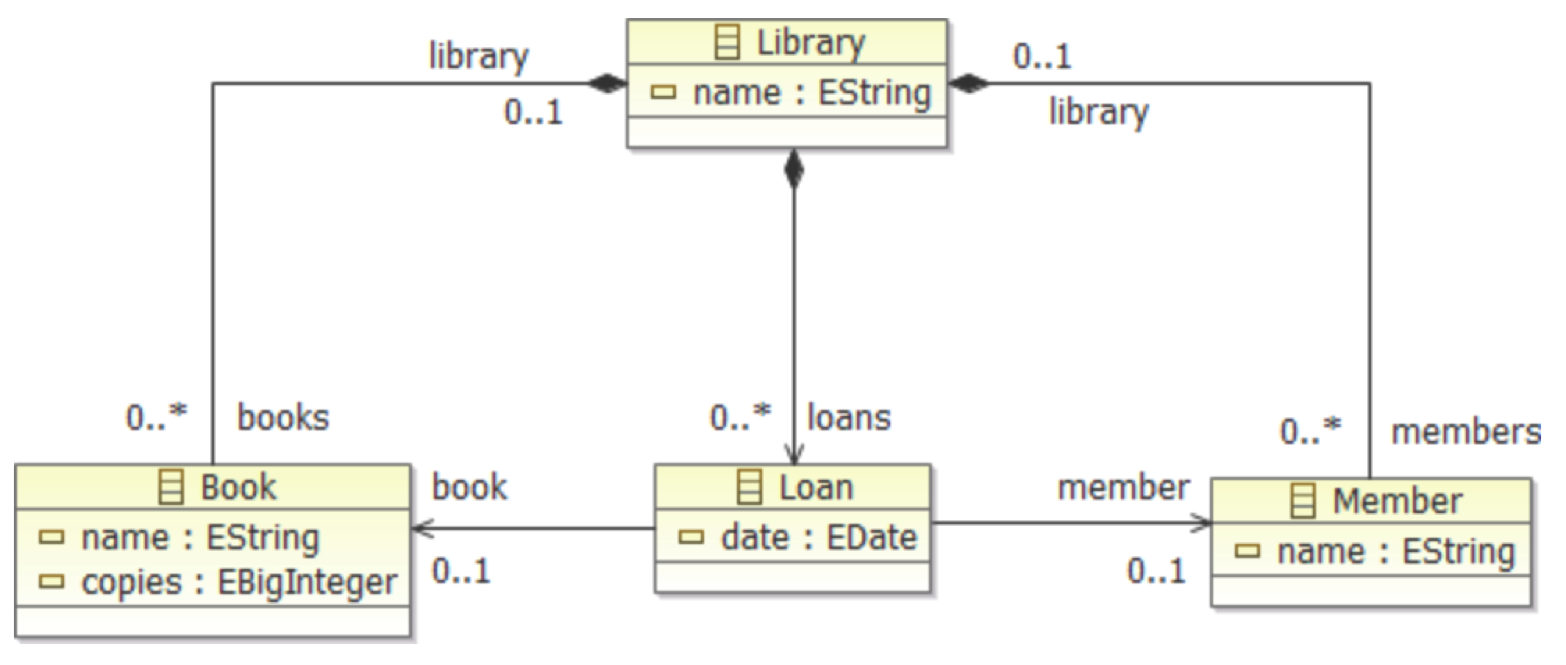
\includegraphics[width=0.9\textwidth]{images/library.png}
\caption{The book library (from \cite{oclinecoreTutorial})}
\label{fig:library}
\end{figure}

\begin{figure}
\begin{schema}{Book}
	name: \seq CHAR \\
	copies: \num
\where
	copies > 0
\end{schema}
\caption{Z model of books in a library}
\label{fig:book-z}
\end{figure}

In many modeling situations such diagrams form the core of the 
modeling effort. Constraints can be added to such diagrams.
For example one constraint could be that the number of copies of a 
book should be a number bigger than or equal to 1. Such a 
constraint can be added inside special constraint box on the 
diagram  in Figure \ref{fig:library}, attached to the \name{Book} 
box with a dotted line. It is interesting to note, that a 
box with an associated constraint (written in another box and linked with a line) conceptually is very similar 
to the idea of a Z schema \cite{Spivey-Z-92}, as shown in Figure 
\ref{fig:book-z}\footnote{Note that the constraint can actually be 
avoided in Z by  defining the type of \izlang{copies} to be $
\mathbb{N}_1$, the natural numbers starting from 1.}.
This schema represents the fundamental concept of a model: a 
signature (the declaration of \izlang{name} and \izlang{copies} above 
the line with their types) and then zero or more axioms (below the 
line). 
%
Attempts have been made to provide textual versions of UML and 
SysML diagrams. An example is  the K specification language 
\cite{havelund-k-modelsward-2016}, that was developed at JPL. 
The expression language of K as well as Z 
(what is written in constraints) is predicate 
logic. Both languages support datatypes such as sets, including 
advanced set expressions such as set comprehension. K is 
object-oriented and is inspired by Z, as well as by
other languages, such as VDM \cite{vdm78,bjoerner-jones-82,jones90,jones-shaw-90,vdmplusplus05} and RAISE \cite{raise92,george-raise-2008,havelund-losl-08}. 

Another textual notation coming out of the model-based engineering community itself is OCLInEcore \cite{oclinecore}, 
which is an attempt 
to define a textual language combining the structure oriented 
Ecore meta-model
of the Eclipse Modeling Framework (EMF)
\cite{emf} with the 
OCL constraint language (Object Constraint 
Language) 
\cite{ocl}. OCL is a declarative expression language that is now 
part of the UML 
standard. OCL descended from Z, but is based on chained method 
calls read from left to right, starting from {\em finite} 
collections, in contrast to predicate logic. For example OCL does 
not have general universal and existential quantification over 
infinite sets. In predicate 
logic we would write a universal quantification over a set/type 
$S$ as follows: $\forall x : S \bullet P(x)$, meaning: for all $x$ 
in the set $S$, $P(x)$ is true. In OCL one would 
write this as:
\iocl{S->forAll(x | P(x))}. However, OCL requires $S$ to be 
finite,
in contrast to predicate logic, where $S$ can be infinite. This
is the major distinction between OCL and predicate logic, in 
addition to the alternative syntax. OCL is executable, given
a model instance.


%The \name{Book} class with the added constraint can be expressed 
%in K as shown in Figure 
%\ref{fig:book-k}, very similar
%to the Z specification. 

%\begin{figure}
%\begin{center}
%\begin{tabular}{c}
%\begin{lstlisting}[language=klang]
%class Book {
%  name : String
%  copies : Int
%   
%  req copies > 0
%}
%\end{lstlisting}
%\end{tabular}
%\end{center}
%\caption{K model of books in a library}
%\label{fig:book-k}
%\end{figure}

In order to illustrate OCLInEcore we expand our example by adding 
the following requirement: ``{\em The number of loans that a book 
is part of should be less than or equal to the 
number of copies of the book}''. The OCLInEcore model 
in Figure \ref{fig:book-oclinecore} formalizes this requirement.
For this purpose, in addition to the two attributes \iocl{name} and \iocl{copies}, two {\em properties} are defined. 
In contrast to an attribute, 
which has a primitive type, a property is linked to one or 
more objects of another user-defined 
type (those drawn as boxes in class diagrams).
The property \iocl{library} links a book to the library it is part 
of, and is the ``{\em opposite property}'' of the \iocl{books} 
property of the \iocl{Library} (expressed using the \iocl{#}-
notation), meaning that if a book is in the \iocl{books} set (a 
bag in fact) of a library, then the library is also in the 
\iocl{library} of the book. The `\iocl{?}' represents 0 or 1.

\begin{figure}
%\begin{center}
%\begin{tabular}{c}
\begin{lstlisting}[language=oclinecore,frame=single,backgroundcolor=\color{light-gray}]
class Book {
  attribute name : String;
  attribute copies : Integer;

  property library#books : Library[?];
     
  property loans : Loan[*] { derived }
  {
    derivation: library.loans->select(book=self);
  }

  operation isAvailable() : Boolean[?]
  {
    body: loans->size() < copies;
  }
     
  invariant CopiesPositive:
    copies > 0;
     
  invariant SufficientCopies:
    loans->size() <= copies;     
}
\end{lstlisting}
%\end{tabular}
%\end{center}
\caption{OCLInEcore model of books in a library (from \cite{oclinecoreTutorial}, modified)}
\label{fig:book-oclinecore}
\end{figure}

The property \iocl{loans} denotes a collection of \iocl{Loan} 
objects and is derived (meaning its value depends on other values), 
with the formula defining 
its value provided as an OCL expression.
The expression reads as follows: from this book (referred to as 
\iocl{self} later in the expression), retrieve the library it is 
part of, retrieve the 
loans of this library, and select those for which the book is 
equal to \iocl{self}. For a given collection \iocl{S}, the 
notation \iocl{S->M(...)} means calling the method \iocl{M} on the 
set \iocl{S}. Hence in this case the
\iocl{select(predicate)} method is defined on sets and returns the 
subset of elements of the set satisfying the predicate.
The two invariants can now be formulated, and their explanation should at this point be straight forward.
The {\em operation} \iocl{isAvailable} is defined to illustrate that one can also define such, here with a body as an 
OCL expression. One can also define operations with side-effects specified with pre/post conditions. No code with side-effects is allowed in 
bodies of operations, which seems to be a limitation, and a sign
of an attempt to move towards a programming language, but not all
the way.

The main point we are trying to make here is that the OCLInEcore 
model, which in reality is very similar to a Z specification 
(signature + axioms), can (for the most part) be elegantly 
expressed in the Scala programming language. This is shown in 
Figure \ref{fig:book-scala}. The class \iscala{Book} extends the
class \iscala{Model}, which we have programmed to offer 
various methods for writing models, including the 
\iscala{invariant} method used to define 
invariants. What in the OCLInEcore model was the property 
\iscala{loans} and the operation \iscala{isAvailable}, are here 
modeled as methods (using the \iscala{def} keyword). 
Multiplicities such as \iocl{Loan[*]} are modeled using Scala's 
collection libraries, in this case \iscala{Set[Loan]}. The Scala 
definitions should be somewhat obvious. It is clear that Scala in 
this case can model this problem in a manner comparable to OCLInEcore. In 
addition, Scala offers so much more than OCLInEcore, such as an 
actual programming language.

\begin{figure}
%\begin{center}
%\begin{tabular}{c}
\begin{lstlisting}[language=scala,frame=single]
trait Book extends Model {
  var name: String
  var copies: Int
  var library: Library

  def loans: Set[Loan] =
    library.loans.filter(_.book eq this)

  def isAvailable(): Boolean =
    loans.size < copies

  invariant("CopiesPositive") {
    copies > 0
  }

  invariant("SufficientCopies") {
    loans.size <= copies
  }
}
\end{lstlisting}
%\end{tabular}
%\end{center}
\caption{Scala program modeling books in a library}
\label{fig:book-scala}
\end{figure}

\begin{figure}[htb]
\begin{center}
\begin{tabular}{c}
\begin{lstlisting}[language=scala]
trait Model {
  type Constraint = Unit => Boolean

  var constraints: List[(String, Constraint)] = Nil

  def invariant(name: String)(c: => Boolean) {
    constraints ::= (name, (Unit => c))
  }

  def verify() {
    for ((n, c) <- constraints) assert(c(), n)
  }
}
\end{lstlisting}
\end{tabular}
\end{center}
\caption{Support for defining invariants in Scala}
\label{fig:invariant-scala}
\end{figure}

The only code that has to be written to provide support for 
writing
class invariants is the definition of the class \iscala{Model}, 
which is shown in Figure \ref{fig:invariant-scala}. Without going 
into details, the class defines a method \iscala{invariant},
which as argument takes a Boolean call-by-name argument. 
The argument is not evaluated before the method body is executed, 
rather, it is only evaluated whenever referred to. In this case
it is stored, still unevaluated, in a list of invariants, all
of which can then be verified on an object of this class 
with a call of \iscala{verify}. Note that such invariants
(specifications) in addition can be the target of more formal analysis, just as they can in a formal specification language.


\subsection{\vdmpp{} Specifications}
\label{sec:vdm-in-scala}

As another example, we shall consider a chemical plant alarm 
management system, first modeled in \vdmpp{} in 
\cite{vdmplusplus05} and also later modeled in Scala in 
\cite{havelund-scala-vdm-12}, which goes into further detail comparing \vdmpp{} and Scala. We show here a slight modification of 
the \vdmpp{} specification as well as the 
corresponding Scala program. In \cite{vdmplusplus05}
the example specification was associated with 
a corresponding UML class diagram to illustrate how the two
techniques can co-exist. Here we shall put emphasis on
\vdmpp{} and its relationship to Scala.

The system shall manage the calling out of experts to deal with 
operational faults discovered in a 
chemical plant. 
Two operations must be provided.
\ivdm{ExpertToPage}: Upon detection of a faulty condition, an 
alarm is raised, and this operation must find an expert on duty 
able to handle the alarm. Each alarm is associated with a specific 
qualification required to fix the causing
problem, and each expert is associated with a set of 
qualifications. Upon an alarm, an expert must be found, and paged, 
that is on duty during the corresponding period and with the right 
qualification.    
\ivdm{ExpertIsOnDuty}: returns the periods during 
which an expert is on duty.      
In addition to providing these two operations, the state of the 
system must satisfy the following
{\em invariant}:
(i) There must be experts on duty during all periods 
allocated in the system. 
(ii) For any alarm and for any period, there should exist an 
expert assigned to that period that has the qualification required
to fix the source problem of the alarm.

The \vdmpp{} class \ivdm{Plant} in Figure \ref{fig:plant-vdm} 
is part of the model of this system (other classes/types shown in
\cite{vdmplusplus05} have been left out here: 
\ivdm{Alarm}, \ivdm{Period}, and \ivdm{Expert}).
The body of this class is divided into three sections: {\em 
instance variables} (mutable variables), {\em functions} (with no 
side-effects), and {\em operations} (with side-effects). An 
invariant defined by the function \ivdm{PlantInv} is imposed on 
the instance variables. The corresponding Scala program modeling the plant is shown in Figure \ref{fig:plant-scala}. We shall not go into the further details, except for mentioning the use of the
\ivdm{suchthat} method, defined in the \ivdm{Model} class, 
which from a finite set selects an element satisfying a predicate provided as argument.

\begin{figure}
%\begin{center}
%\begin{tabular}{c}
\begin{lstlisting}[language=vdm,frame=single,backgroundcolor=\color{light-gray}]
class Plant
  instance variables
    alarms : set of Alarm;
    schedule : map Period to set of Expert;
    
    inv PlantInv(alarms,schedule);

 functions
    PlantInv: set of Alarm * map Period to set of Expert -> bool
    PlantInv(as,sch) ==
      (forall p in set dom sch & sch(p) <> {}) and
      (forall a in set as &
         forall p in set dom sch & 
           exists expert in set sch(p) &
             a.GetReqQuali() in set expert.GetQuali());

  operations
    public ExpertToPage: Alarm * Period ==> Expert
    ExpertToPage(a, p) ==
      let expert in set schedule(p) be st
        a.GetReqQuali() in set expert.GetQuali()
      in
        return expert
    pre a in set alarms and p in set dom schedule
    post let expert = RESULT in
      expert in set schedule(p) and
      a.GetReqQuali() in set expert.GetQuali();
		
		 
    public ExpertIsOnDuty: Expert ==> set of Period
    ExpertIsOnDuty(ex) ==
      return {p | p in set dom schedule & ex in set schedule(p)};
end Plant
\end{lstlisting}
%\end{tabular}
%\end{center}
\caption{\vdmpp{} model of plant}
\label{fig:plant-vdm}
\end{figure}

\begin{figure}
%\begin{center}
%\begin{tabular}{c}
\begin{lstlisting}[language=scala,frame=single]
trait Plant extends Model {
  var alarms: Set[Alarm]
  var schedule: Map[Period, Set[Expert]]

  invariant{PlantInv(alarms, schedule)}

  def PlantInv(alarms: Set[Alarm], schedule: Map[Period, 
  Set[Expert]]): Boolean =
    (schedule.keySet forall {p =>  schedule(p) != Set() }) &&
      (alarms forall { a =>
        schedule.keySet forall { p =>
          schedule(p) exists { expert =>
            a.reqQuali in expert.quali
          }
        }
      })


  def ExpertToPage(a: Alarm, p: Period): Expert = {
    require((a in alarms) && (p in schedule.keySet))
    schedule(p) suchthat { expert =>
      a.reqQuali in expert.quali
    }
  } ensuring { expert =>
    (a.reqQuali in expert.quali) &&
      (expert in schedule(p))
  }

  def ExpertIsOnDuty(ex: Expert): Set[Period] =
    schedule.keySet filter { p => ex in schedule(p) }
}
\end{lstlisting}
%\end{tabular}
%\end{center}
\caption{Scala program modeling plant}
\label{fig:plant-scala}
\end{figure}

\subsection{Domain-Specific Languages}
\label{sec:dsl-in-scala}

We consider the ability to define domain-specific languages (DSLs) 
an essential part of a modeling/programming framework. This form of 
activity is supported 
within the UML/SysML community through meta-modeling and profiles. 
Programming languages have been slower to pick up this concept, 
although an early language such as LISP supported macros
from its birth. A modern programming language such as Scala 
supports definition of
so-called {\em internal} DSLs with a collection of a few 
elegant language features. In this section we shall illustrate this 
with an example
DSL for monitoring event sequences. 
The example was also listed in \cite{havelund-joshi-experience-2014}.
An {\em internal} DSL is an extension of the programming language, 
in this case 
effectively an API, however, expressed in such a way that use of 
this API
has the flavor of new syntax added to the language.

\begin{figure}
%\begin{center}
%\begin{tabular}{c}
\begin{lstlisting}[language=scala,frame=single]
class NoLockCycles extends Monitor {
  "r1" -- 'acquire('t,'l) |-> 'Locked('t,'l)
  "r2" -- 'Locked('t,'l) & 'release('t,'l) |-> remove('Locked)
  "r3" -- 'Locked('t,'l1) & 'acquire('t,'l2) |-> 'Edge('l1,'l2)
  "r4" -- 'Edge('l1,'l2) & 'Edge('l2,'l3) & not('Edge('l1,'l3)) |-> 'Edge('l1,'l3)
  "r5" -- 'Edge('l1,'l2) |-> { if (get('l1) == get('l2)) fail() }
}
\end{lstlisting}
%\end{tabular}
%\end{center}
\caption{Scala program written in the rule DSL, 
monitoring lock operations}
\label{fig:deadlocks-scala}
\end{figure}

The DSL illustrated here is the LogFire \cite{havelund-logfire-sttt14},
created for rule-based programming, and specifically for 
writing temporal trace properties. We shall not go into the details of LogFire (the reader is referred to \cite{havelund-logfire-sttt14}), but only show a model written in this DSL, 
and briefly explain how the DSL is defined. 
A monitor is specified as a set of rules, each of the form: 

\[
  \textit{name}\ \verb+--+\ \textit{condition}_1\ \& \ldots \&\ \textit{condition}_n\ \longmapsto\  \textit{action}
\]

\noindent
A rule consists of a left-hand side: a list of conditions, and a 
right-hand side:
an action. The rules operate on a set of facts, the 
{\em fact memory} (implemented as a RETE network \cite{forgy-rete-82}) 
where conditions check the presence or absence of certain facts, 
and the action adds or deletes 
facts, or execute any Scala code inserted as an action. Figure 
\ref{fig:deadlocks-scala} illustrates 
a monitor, which monitors $acquire(thread,lock)$ and 
$release(thread,lock)$ events emitted from an instrumented 
multi-threaded application, that uses locks to protect against
data races. The monitor attempts to determine whether any 
group of threads access locks
in a cyclic manner, which potentially can lead to deadlocks (the classical dining philosopher problem). 
A cycle is detected if for any lock $l$ there is 
an edge from $l$ back to itself.

The class contains five rules. Beyond the monitored events
\iscala{acquire} and \iscala{release}, the monitor adds 
and deletes \iscala{Locked(thread,lock)} facts (the thread holds
the lock), and adds \iscala{Edge(lock1,lock2)} facts, representing
that there is an edge from \iscala{lock1} to \iscala{lock2}, indicating that a thread holds  \iscala{lock1} while acquiring
\iscala{lock2}. The class extends the \iscala{Monitor} class which contains the DSL definitions that allow us to write rules in this manner. Specifically the functions: \iscala{--}, \iscala{&}, \iscala{|->}, \iscala{remove}, and \iscala{fail}. 

The implementation of this DSL relies on Scala's (1) 
allowance for methods having symbol names, such as \iscala{--}
and \iscala{|->}, (2) allowance for method calls of the form 
\iscala{obj.method(arg)} to be written as 
\iscala{obj method arg}, and (3) automated insertion (by 
the compiler) of 
user-defined {\em implicit} 
functions that can lift a value of one type 
to a value of another type in places where the compiler's type 
checker fails to type check an expression. For example part of
the DSL implementation are the definitions shown in Figure
\ref{fig:dsl-scala}.
The implicit function \iscala{liftRuleName} 
gets invoked by the compiler automatically when a string is 
followed by the symbol \iscala{--}. It lifts the string (rule name) to an anonymous object, which provides the method \iscala{--}, which when applied to a condition returns
an \iscala{RuleDef} object, which provides the methods \iscala{&}
and \iscala{|->}. This way method calls can be chained together.

\begin{figure}
\begin{center}
\begin{tabular}{c}
\begin{lstlisting}[language=scala]
implicit def liftRuleName(name: String) = 
  new { 
    def --(c: Condition) = new RuleDef(name, List(c)) 
  }

class RuleDef(name: String, conditions: List[Condition]) { 
  def &(c: Condition) = new RuleDef(name, c :: conditions)

  def |->(stmt: => Unit) { 
    addRule(Rule(name, conditions.reverse, Action((x: Unit) => stmt))) 
  } 
}
\end{lstlisting}
\end{tabular}
\end{center}
\caption{Scala rule DSL implementation}
\label{fig:dsl-scala}
\end{figure}

We do notice, however, some drawbacks of the Scala DSL.
Notice the quoted names: \iscala{'acquire}, \iscala{'Locked}, 
\iscala{'t}, etc. These are Scala symbols (elements of the type 
\iscala{Symbol}). It is not possible in this form of DSL to avoid 
these quotes. Likewise, the name of the rule is a string. 
Furthermore, a monitor in this DSL cannot be type checked without 
actually running the monitor. That is to say, Scala's DSL defining
features are not optimal, although they do make defining internal 
DSLs somewhat easier.


\section{Discussion and Conclusion}
\label{sec:conclusion}


\label{sec:concerns}

A unified modeling and programming framework has to satisfy 
quite different and contradicting goals.
First of all, it has to represent the concepts of the 
application domain at an adequate level of 
abstraction such that the specialities of the applications 
are directly represented and not covered by awkward implementation 
concepts.  
Second it has to address the structuring of algorithms and data 
structures in a way such that programs stay understandable, 
modular and support the most important methods of structured 
program development. And finally it has to allow addressing 
specific implementation properties of execution machines including 
their operating systems, such that it can be controlled how the 
implementation uses resources and exploits the possibilities of 
the execution platform and its hardware. An obvious problem here 
of course is to what extent the particular application domain 
influences the programming language, and to what extent this 
is true for the execution platform and efficiency concerns as
well. In the following we shall briefly mention some of the
elements to consider when imagining a unified approach to
modeling and programming.


\subsubsection{Target domains}

We can observe three major domains of interest, namely modeling; 
programming of non-embedded systems, such as web applications, 
including scripting; and finally programming of embedded/cyber-
physical systems. It is clear that these three domains till date 
have been addressed by different communities and different 
languages. The question is to what extent these
quite different domains could be targeted with the same formalism.
Note that the different modeling and programming languages used on
different targets have an overwhelming number of language constructs in
common, to an extent where this question at least needs to be answered
in a scientific manner rather than in an opinionated emotional manner.

\subsubsection{Predicate specifications}

A formalism must generally support specifying properties as 
predicates rather than only as algorithms. Predicate-oriented techniques 
include design-by-contract, including pre- and post-conditions, as 
well as state invariants. Such can for example be found in Eiffel 
as  well as in SPARK. This concept can be carried 
further to for example include behavioral sequence specification, 
such as temporal logics, sequence diagrams, etc.
Note, however, that many models are very operational in
nature, and hence can very well best be formulated as state 
machines, or programs (data structures and algorithms). 

\subsubsection{Programming in the large}

A formalism must support programming in the large, and in general
provide good modularization and component-based development. One cannot discuss components without discussing concurrency. Concurrency is an essential part of modern programming, especially 
considering the emergence of multi-core computers. However, 
concurrency is important at the modeling level as well, where it 
can serve as a natural way to describe interacting agents. 
Important concepts include agent systems, message passing based 
communication, parallel data structures (programming concurrent 
without knowing it), and distributed programming.

\subsubsection{High-level programming}

A formalism must support high-level programming as found in modern
programming languages. The elegance  of functional programming has 
been praised many times. Nevertheless its breakthrough is only 
recent. In contrast, object-oriented programming, 
which in particular addresses encapsulation and reuse, has been very 
popular for decades now. A language such as Scala 
integrates the two paradigms nicely, as even early versions 
of LISP (CLOS) did. 
Functional programming means for example functions as 
values (lambda abstractions) and pattern matching, and of course 
reliance on recursion. Functional programming is by some considered 
the best approach to use multi-core systems due to no shared state 
updates. A key feature of VDM was the introduction of elegant syntax for collections, such as sets, lists and maps. These days such concepts are introduced in languages mostly as libraries. Fortress has built-in syntax for these very similar to VDM.
There should be easy ways of iterating through collections – to avoid indexing problems, as well as support for parallel computation over such.
A formalism should be statically typed, although with type inference, and with allowance for going type less
in clearly defined regions to support scripting. 
Decades of experience in strong type systems should be harvested, including more recent  topics such as dependent types, session types, and units.

\subsubsection{Low-level programming}

A formalism must support low-level programming.
Embedded programing often means: no dynamic memory 
allocation after initialization, no garbage collection, some 
knowledge of memory layout, even to the point where computation 
with addresses is used to improve speed. This again means use of 
low level programming languages such as C. C, however, allows for 
memory errors and makes programmers less effective as they would 
otherwise be were they allowed to program in higher-level 
languages. We need to satisfy the needs encountered by typical C 
programmers, including offering comparable speed and memory 
control. This includes support for hardware control and
targeting specific execution platforms 


\subsubsection{Continuous mathematics}

A formalism must support modeling of cyber-physical systems. That
is: physical systems controlled by computer programs. To model (not program) a cyber-physical system, there is a need for describing
continuous behavior using continuous mathematics, including
for example differential equations, as supported by for example
Modelica \cite{?}. Modelica is an object-oriented  
language for modeling systems containing mechanical, electrical, electronic, hydraulic, thermal, control, electric power or process-oriented subcomponents. Models can be simulated.
Similar tools are: Mathematica \cite{?} and
MATLAB \cite{?}.


\subsubsection{Domain-specific languages}

A formalism must support definition of DSLs (Domain-Specific 
Languages). A key to modeling and programming is to capture 
the relevant concepts of the application domain. UML for example
supports meta-modeling and profiles, used for defining (graphical)
DSLs. The programming language community is still somewhat behind
in this respect. It should be easy for developers to define new
DSLs either external stand-alone, or internal extending the
modeling/programming formalism.

\subsubsection{Visualization}

A formalism must be visualizable.
Visualization is of extreme importance, as demonstrated by the 
relative success of formalisms such as UML and SysML in the 
engineering community, when compared 
to formal methods textual notations. People generally are more at 
ease looking at a 2-dimensional illustration when they encounter a 
problem specification for the first
time, and it eases communication. Whether visualization is useful 
as well for entering
and maintaining specifications is another matter. We do believe 
that visualization and 
text should match up, such that modification of one leads to 
immediate change in the 
other. Visualization is normally static, rendering static models as
pictures. However, visualization can also be dynamic, of program 
executions, illustrating how behavior evolves.

\subsubsection{Analysis}

A formalism must be analyzable.
A key concept in a combined modeling and programming environment is 
the support for advanced analysis of models/programs, including, 
but also beyond, what is normally supported in standard programming 
environments. This ranges from basic built-in support for unit 
testing, over advanced testing capabilities, including test input 
generation and monitoring, to concepts such as static analysis, 
model checking, theorem proving and symbolic execution. A core 
requirement, however, must be the practicality of these solutions. 
The main emphasis should be put on automation. The average user 
should be able to benefit from automated verification, without 
having to do manual proofs. However, support for manual theorem 
proving should also be possible, for example for core critical 
algorithms. Integration of static and dynamic analysis will be 
desirable: verify what is practically feasible, and test (monitor) 
the remaining proof obligations.

\subsubsection{Conclusion}

We have in this paper outlined some views on the potential in 
combining modeling and programming, supported by analysis 
capabilities such as static analysis, model checking, theorem 
proving, monitoring, and testing. We believe that the time is right 
for the formal methods/modeling and programming language 
communities to join forces. To some extent this is already 
happening in the small. However, we believe that we are standing in 
front of a major wave of research creating a united foundation for 
modeling, programming and verification. A cynical argument is that 
this is all obvious, which may very well be true. 

\bibliography{bib}
\bibliographystyle{abbrv}

\appendix


\section{Websites}

\subsection{Modeling}

\begin{itemize}
\item CIP: http://en.wikipedia.org/wiki/Wide-spectrum\_language
\item Coq: https://coq.inria.fr
\item JML: http://www.eecs.ucf.edu/~leavens/JML//index.shtml
\item Mathematica: http://www.wolfram.com/mathematica
\item Modelica: https://www.modelica.org
\item OBJ: http://c2.com/cgi/wiki?ObjLanguage
\item PVS: http://pvs.csl.sri.com
\item RAISE: http://spd-web.terma.com/Projects/RAISE
\item SysML: http://www.omgsysml.org
\item TLA: http://research.microsoft.com/en-us/um/people/lamport/tla/tla.html
\item UML: http://www.uml.org
\item VDM: http://en.wikipedia.org/wiki/Vienna\_Development\_Method
\item Z: http://en.wikipedia.org/wiki/Z\_notation
\end{itemize}

\subsection{Programming}

\begin{itemize}
\item Agda: http://wiki.portal.chalmers.se/agda/pmwiki.php
\item C: http://en.wikipedia.org/wiki/C\_(programming\_language)
\item C\#: https://msdn.microsoft.com/en-us/library/67ef8sbd.aspx
\item D: http://dlang.org
\item Dafny: http://research.microsoft.com/en-us/projects/dafny
\item Eiffel: https://www.eiffel.com
\item F\#: http://fsharp.org
\item Fortress: java.net/projects/projectfortress/pages/Home
\item Go: https://golang.org
\item Haskell: https://www.haskell.org
\item Java: https://www.oracle.com/java/index.html
\item JavaScript: http://www.w3schools.com/js/
\item LISP (CLOS): http://www.cs.cmu.edu/Groups/AI/html/cltl/cltl2.html
\item Ocaml: http://caml.inria.fr/ocaml
\item Python: https://www.python.org
\item Ruby: https://www.ruby-lang.org/en
\item RUST: http://www.rust-lang.org
\item Scala: http://www.scala-lang.org
\item SPARK: http://libre.adacore.com/tools/spark-gpl-edition
\item Spec\#: http://research.microsoft.com/en-us/projects/specsharp
\item Swift: https://developer.apple.com/swift
\end{itemize}

\end{document}
